\chapter[Synch array]{synch array}
\section{Introduction}

Many communication systems use a substitution-error correcting
code to encode a binary input message $\mathbf{x}$ into a coded
sequence $\mathbf{c}$ = $C(\mathbf{x})$. The modulated version of
this sequence, corrupted by additive noise, arrives at the
receiver as a waveform $r(t)$,
\begin{equation}\label{eq:rt}
r(t)=\sum_{i} c_i h(t-iT) +n(t),
\end{equation}
where $c_i$ is the $i^{\text{th}}$ %$i^{\text{th}}$
bit of $\mathbf{c}$, $h(t)$ is the modulating pulse, and $n(t)$ is
the noise introduced in the channel.

Upon receiving $r(t)$, the receiver samples it at the times
$\left\{kT_s+\tau_k\right\} $. The samples are fed into the
decoder which produces the most likely input message. In
traditional correlation based receivers, for adequate noise
rejection, it is essential that the decoder be provided with
samples taken at approximately optimal time instances. As the
operating requirements under which timing recovery must be
performed become more stringent, such as lower signal to noise
ratio (SNR) and higher data rates, accurate synchronization
becomes critical for the full utilization of the available coding
gains.

Several authors have studied the problem of accurate timing
recovery in such challenging environments. Proposed solutions
include building a more sophisticated timing recovery block
\cite{liu:02}, a turbo-like approach to iteratively determine both
sampling points and encoded data \cite{mcla:02}, and multiple
hypothesis analysis of the sampling instances \cite{kbek:04}.

As an alternative to more complex and more expensive timing
recovery schemes, we propose to instead modify the decoding
procedure and the code itself to compensate for imperfect
synchronization. The rationale of this approach is that, after a
systematic analysis of the robustness of the code to
synchronization errors, one could use a subcode of it that would
be immune to both substitution as well as synchronization errors.
The incurred rate loss in the proposed approach would need to be
traded off against the increased complexity and latency associated
with the earlier mentioned approaches. The challenge of the
proposed approach lies in understanding the synchronization error
correction capabilities of given codes of interest by determining
high rate subcodes with adequate immunity to synchronization
errors.

To emphasize the issues that arise when adequate timing recovery
is missing, assume that the modulation scheme in (\ref{eq:rt}) is
pulse-amplitude modulation (PAM), and more importantly, that we
are operating in the infinite SNR regime where the effect of
$n(t)$ is negligible. As a consequence of the initial frequency
error, say when $T_s < T$, or of the accumulated phase error in
$\tau_k$, some symbol may be sampled more than once (effectively
repeated in the infinite SNR regime)\footnote{The case $T_s>T$
that may also be of interest is not considered here. See
\cite{techRM:06} for related work.}.

A codeword $\mathbf{c}$ can thus give rise to a whole set of
received sampled versions of $r(t)$. We will assume that the
number of samples is known, so that codewords can be analyzed in
isolation. Thus, for instance, if there is one repetition,
$\mathbf{c}$ can give rise to the set $R_1(\mathbf{c})$ of all
strings obtained by applying a repetition to $\mathbf{c}$. When
two distinct sequences $\mathbf{c_1}$ and $\mathbf{c_2}$ result in
the same sampled sequence, it is no longer possible to uniquely
determine the codeword or its pre-image $\mathbf{x}$ from the
received sequence, \textit{even in the noise-free environment}. We
then say that the code $C(n,k)$ suffers from an
\textit{identification problem}. We also say that the pair of
distinct codewords $\mathbf{c_1}$ and $\mathbf{c_2}$ suffers from
an identification problem. For the one repetition case, for
instance, this occurs when $R_1(\mathbf{c_1}) \bigcap
R_1(\mathbf{c_2})$ is nonempty.

Several authors have studied codes immune to a deletion or an
insertion of a bit. For example, the so-called
Varshamov-Tenengolts code proposed in \cite{vt:65} and popularized
by Levenshtein in \cite{lev:66} has been further studied in
\cite{sloane:00}. A related construction has been proposed in
\cite{klove:95}. While providing immunity to the deletion or
insertion of a bit, such constructions do not generally guarantee
other desirable properties over a channel that introduces
substitution errors, such as linearity, good minimum Hamming
distance, and efficient encoding/decoding algorithms. Concatenated
codes that correct synchronization and substitution errors have
been proposed in \cite{cmnv:03} and \cite{dmackay:01}, but suffer
from a significant loss in rate.

In this paper we first present a brief overview of the array-based
LDPC codes and discuss their identification properties. In Section
\ref{sec3} we propose a general technique for constructing
collections of binary strings immune to multiple repetitions.
Having established several useful ancillary results in Section
\ref{aux}, we then describe in Section \ref{enc} how the
array-based LDPC code can be modified to eliminate the
identification problem for the single repetition model. A decoding
algorithm appropriate for channels with a single repetition and
substitution
errors is developed in Section \ref{dec}. %\textbf{to be changed}
\section{Array-based LDPC codes}\label{ldpc}

Array based LDPC codes are regular LDPC codes parameterized by
integers $j$ and $p$, where $1 \le j \leq p$, and $p$ is an odd
prime, having the parity check matrix $H_{p,j}$ given by
(\cite{mittel:02}) \small\begin{equation}\label{eq:1}
H_{p,j}=\left[\begin{array}{ccccc}
I & I & I & \ldots & I\\
I & \sigma & \sigma^2 & \ldots &\sigma^{p-1}\\
I & \sigma^2 & \sigma^4 & \ldots &\sigma^{2(p-1)}\\
\vdots & \vdots & \vdots & \ldots & \vdots \\
I & \sigma^{j-1} & \sigma^{(j-1)2} & \ldots &\sigma^{(j-1)(p-1)}\\
\end{array}
\right]
\end{equation}\normalsize
where $\sigma$ denotes a $p \times p$ permutation matrix
circularly shifted by 1 position, i.e. \small
\begin{equation}
\sigma=\left[\begin{array}{ccccc}
0 & 0 & \ldots & 0 & 1\\
1 & 0 & \ldots & 0 & 0\\
0 & 1 & \ldots & 0 & 0\\
\vdots & \vdots & \ldots & \vdots & \vdots\\
0 & 0 & \ldots & 1 & 0\\
\end{array}
\right].
\end{equation}
\normalsize We let $C_{p,j}$ denote the linear code with the
parity check matrix given in (\ref{eq:1}). Note that $H_{p,j}$ is
of rank $pj - j +1$.

Array-based LDPC codes have good performance \cite{fan} and low
encoding complexity \cite{mittel:02}. They have been proposed for
a variety of applications, including digital subscriber lines
\cite{ibm:02} and magnetic recording applications \cite{kumar:04}.
These codes permit efficient parallel decoding. However, as
explained below, they suffer from an identification problem.

\begin{lemma} \textit{Under the single repetition model,
there are at least $2^{p-2}-1$ identification problem causing
codeword pairs in $C_{p,j}$ for $1< j <p$.}\end{lemma}

\textit{Proof}: Let $\mathbf{c_1}$ denote
$[a_2a_3...a_{p-2}a_{p-1}\overline{a}_pa_1]$ and $\mathbf{c_2}$
denote $[a_3a_4...a_{p-1}a_p\overline{a}_1a_2]$, where $a_i$
($\overline{a}_i$) denotes a string of length $p$ bits with a
single 1 (0) in the $i^{\text{th}}$ position and 0's (1's)
everywhere else.

%For example, for $p=5$, $\mathbf{c_1}$ is [01000 00100 00010 11110
%10000] and $\mathbf{c_2}$ is [00100 00010 00001 01111 01000].

We see that $\mathbf{c_1}$ and $\mathbf{c_2}$ can both give rise
to the same string after one repetition, namely
$[a_3a_4...a_{p-1}a_p\overline{a}_1a_20]$ (same as
$[0a_2a_3...a_{p-2}a_{p-1}\overline{a}_pa_1]$). %For example, for
%$p=5$, $\mathbf{c_1}$ and $\mathbf{c_2}$ can both result in [00100
%00010 00001 01111 010000].

We now prove that $\mathbf{c_1}, \mathbf{c_2}$ are in fact
codewords of $C_{p,p-1}$.

Let $\mathbf{c_1}^{\langle kp \rangle}$ denote the string obtained
by cyclically shifting $\mathbf{c_1}$ to the right by ${kp}$
positions. Since $C_{p,j}$ is quasi-cyclic \cite{mittel:02}, it
suffices to verify that $\mathbf{c_1}^{\langle 2p
\rangle}$=$[\overline{a}_pa_1a_2a_3...a_{p-2}a_{p-1}]$ and
$\mathbf{c_2}^{\langle 2p
\rangle}$=$[\overline{a}_1a_2a_3a_4...a_{p-1}a_{p}]$ satisfy
$\mathbf{c_1}^{\langle 2p \rangle}H_{p,p-1}^T=0$ and
$\mathbf{c_2}^{\langle 2p \rangle}H_{p,p-1}^T=0$.

It is easily seen that $\mathbf{c_1}^{\langle 2p
\rangle}[II...I]^T=0$. Now consider a row-wise submatrix $[I
\sigma^l \sigma^{2l} \dots \sigma^{l(p-1)}]$ of $H_{p,p-1}$,  for
some $l$, $1 \leq l \leq p-2$. Write $\mathbf{c_1}^{\langle 2p
\rangle}[I \sigma^l \sigma^{2l} \dots\sigma^{l(p-1)}]^{T}$ as
$\overline{a}_p +\sum_{i=1}^{p-1} a_i [\sigma^{il}]^T$ =
$\overline{a}_p +\sum_{i=1}^{p-1} a_{[i+il]_p}$, where $[x]_p$
indicates $x$ mod $p$. Since $1 \leq i \leq p-1$ and $1 \leq l
\leq p-2$, $(i+il)$ mod $p \neq$ 0, and no term in the summation
is $a_p$. In addition, all terms in the summation are distinct, as
otherwise there would exist $i,i'$, $i' < i$ such that
$(i-i')(l+1) \equiv 0 $ mod $p$, which is impossible for $p$
prime, $i,i' \leq p-1$ and $l+1 \leq p-1$. Therefore,
$\mathbf{c_1}^{\langle 2p \rangle}[I \sigma^l \sigma^{2l}
\dots\sigma^{(p-1)l}]^{T}=0$. The proof for $\mathbf{c_2}^{\langle
2p \rangle}H_{p,p-1}^T=0$ is analogous.


Provided that both $\mathbf{c_1}^{\langle kp \rangle}$ and
$\mathbf{c_2}^{\langle kp \rangle}$ have the same starting and
ending bits, they too suffer from the identification problem in
the single repetition model. This occurs as long as $k$ is not
congruent to 1 or to 2 mod $p$. Let $B_{1}$ ($B_{2}$) be the set
of codewords obtained by cyclically shifting $\mathbf{c_1}$
($\mathbf{c_2}$) by $kp$ positions for $k$ ranging from $3$ to
$p$. One can directly check that the pair comprised of any
nontrivial linear combination of elements in $B_{1}$ and the same
linear combination of their counterparts in $B_{2}$ also suffers
from the identification problem.

Since, by construction, $C_{p,j} \supseteq C_{p,j+1}$, in each
$C_{p,j}$ there are therefore at least $2^{p-2}-1$ pairs of
codewords suffering from the identification problem.
%One can also check that
%different linear combinations of the elements of $B_{1}$ and $B_{2}$
%result in different codewords. \hfill $\blacksquare$

\section{Construction of a multiple
repetitions correcting set}\label{sec3}

For a binary string $\mathbf{s}$, let $R_t({\mathbf{s}})$ denote
the set of all strings obtained by applying $t$ repetitions to
$\mathbf{s}$. We call a collection $S$ of strings $t$-repetitions
correcting if the sets $R_t(\mathbf{s_1})$ and $R_t(\mathbf{s_2})$
are disjoint for all distinct elements $\mathbf{s_1},
\mathbf{s_2}$ of $S$. In this section we describe a method for
constructing a $t$-repetitions correcting collection of strings,
building on the $t=1$ case \cite{lev:66}, \cite{sloane:00}. Given
a code, this can in principle be used to develop a subcode that
does not suffer from the identification problem for $t$
repetitions, along the lines developed for $t=1$ in Sections
\ref{enc} and \ref{dec}.

Let us first introduce a useful transformation in which we express
the number of runs of a string in terms of the weight of a string
in the transformed domain. For a string $\mathbf{c}$ of length
$n$, let the string $\tilde{\mathbf{c}}$ of length $n-1$ be
defined as $\mathbf{c}T_n$, where $T_n$ is a $n \times (n-1)$
matrix
satisfying\vspace{-0.0in}\begin{equation}\label{eq:t}T_{n}(i,j)=\left\{
\begin{array}{lll}
    1, & \text{if }i = j,j+1\\
    0, & \text{else.} \\
\end{array} \right. \end{equation}
If $\mathbf{c}$ has $r$ runs, then $\mathbf{\tilde{c}}$ has weight
$r-1$, and vice versa. Both $\mathbf{c}$ and its complement
$\mathbf{\overline{c}}$ result in the same $\mathbf{\tilde{c}}$.

If $C$ is a linear code of length $n$ with a generator matrix $G$,
its image under $T_n$ is a linear code generated by
$\tilde{G}=GT_n$. If the all-ones is not a codeword in $C$, then
$\tilde{G}$ is full rank.

A repetition in $\mathbf{c}$ corresponds to an insertion of a zero
in its counterpart $\mathbf{\tilde{c}}$. Therefore, to construct a
collection of strings that is $t=1$ repetition correcting, it
suffices to construct a collection of strings that is single
insertion of a zero correcting in the transformed domain.

For $w \geq 1$, consider the set $S(m,w,a,r)$ defined as:
%\vspace{-0.2in}
\begin{equation}\label{s1}\begin{array}{ll}S(m,w,a,r)= \{ & \mathbf{s}=(s_1, s_2, ... s_m) \in \{0,1\}^m
:\\
{} & \sum_{i=1}^m s_i = w, \sum_{i=1}^m is_i \equiv a  \text{ mod
}r \}.\end{array}\end{equation} The set $S(m,0,0,r)$ contains just
the all zeros string by convention. Let $a_0 = 0$, and let
$S\left(m,(a_1,r_1),(a_2,r_2),...,(a_m,r_m)\right)$ be defined as
\vspace{-0.1in}
\begin{equation}\label{union1}S\left(m,(a_1,r_1),(a_2,r_2),...,(a_m,r_m)\right)=
\bigcup_{l=0}^{m} S(m,l,a_l,r_l).\end{equation}
\begin{lemma}\label{lemma2}\textit{Provided that $r_l >l$ $\forall l \in [0,m]$, the
set $S\left(m,\left(a_1,r_1\right),(a_2,r_2),...,(a_m,r_m)\right)$
is single insertion of a zero correcting.}\end{lemma}


\textit{Proof}: If each set in the disjoint union in
(\ref{union1}) is single insertion of a zero correcting, so is
their (disjoint) union. Consider $\mathbf{x} \in S(m,l,a_l,r_l)$
for $r_l > l$. Following the analysis in \cite{lev:66},
\cite{sloane:00}, suppose the insertion of a zero occurs in the
$L^{\text{th}}$ position (which is unknown). Let $\mathbf{x'}$
denote the resulting string. Compute $a' \equiv$ $\sum_{i=1}^m
ix_i'$ mod $r_l$;
\begin{equation}\begin{array}{lll}a'
& \equiv \sum_{i=1}^m ix_i' \text{ mod } r_l \\
{} & \equiv \left(\sum_{i=1}^{L-1} ix_i+ \sum_{i=L}^{m}
(i+1)x_i\right) \text{ mod }r_l\\ {} & \equiv \left(a_l+R
\right)\text{ mod }r_l,\end{array}\end{equation} where $R$ denotes
the number of ones to the right of the inserted 0. Since $R \leq l
< r_l$, the offset $R$ mod $r_l$ can be uniquely determined from
$a_l$ and $a'$ mod $r_l$, and the string $\mathbf{x}$ is recovered
by deleting a zero immediately preceding the $R^{\text{th}}$ 1 in
$\mathbf{x'}$ counting from the right.\hfill$\blacksquare$


The construction given in (\ref{s1}) and (\ref{union1}) can be
generalized for the correction of multiple repetitions as follows:

Let $w$ denote the weight of $\mathbf{s}$, let
$b_{i+1}=b_{i+1}(\mathbf{s})$, $1 \leq i \leq w$ be the size of
the run of zeros immediately following the $i^{\text{th}}$ 1 in
$\mathbf{s}$, and let $b_1=b_1(\mathbf{s})$ be the size of the run
of zeros preceding the leftmost 1. If the $i^{\text{th}}$ 1 is
immediately followed by another 1, $b_{i+1}=0$, and if the
leftmost bit in $\mathbf{s}$ is 1, $b_1=0$. Moreover, if
$\mathbf{s}$ consists only of zeros, $b_1=$ length of
$\mathbf{s}$. We call $b_i$ the size of the $i^{\text{th}}$ bin of
zeros of $\mathbf{s}$.

Let $\mathbf{a}=\left(a_1,a_2,...,a_t\right)$ for $t \geq 1$, and
consider the set $\hat{S}(m,w,\mathbf{a},p)$ for $w \geq 1$
defined as
\begin{equation}\begin{array}{lll}\hat{S}(m,w,\mathbf{a},p) = \{ & \mathbf{s}=(s_1, s_2, ... s_m) \in \{0,1\}^m
:\\ {} & \sum_{i=1}^m s_i = w,\\
{} & \sum_{i=1}^{w+1} ib_i \equiv a_1 \text{ mod } p,\\ {} &
\sum_{i=1}^{w+1} i^2b_i
\equiv a_2 \text{ mod } p,\\
{} & \hspace{0.5in}\vdots\\ {} & \sum_{i=1}^{w+1} i^tb_i \equiv
a_t \text{ mod } p\}.\end{array}\end{equation} The set
$\hat{S}(m,0,\mathbf{0},p)$ contains just the all-zeros string by
convention. Let $\mathbf{a_0} = \mathbf{0}$ and let
$\hat{S}\left(m,(\mathbf{a_1},p_1),(\mathbf{a_2},p_2),...,(\mathbf{a_m},p_m)\right)$
be defined as \vspace{-0.1in}
\begin{equation}\label{union}\hat{S}\left(m,(\mathbf{a_1},p_1),(\mathbf{a_2},p_2),...,(\mathbf{a_m},p_m)\right)=
\bigcup_{l=0}^{m} \hat{S}(m,l,\mathbf{a_l},p_l).\end{equation}
\begin{lemma}\textit{If each $p_l$ is prime and $p_l >$
max$(t,l)$, the set
$\hat{S}\left(m,(\mathbf{a_1},p_1),(\mathbf{a_2},p_2),...,(\mathbf{a_m},p_m)\right)$
is t-insertions of zeros correcting.}\end{lemma}

\textit{Proof}: It suffices to show that each set
$\hat{S}(m,l,\mathbf{a_l},p_l)$ is $t$-insertions of zeros
correcting. Consider $\mathbf{x} \in$
$\hat{S}(m,l,\mathbf{a_l},p_l)$. After experiencing $t$ insertions
of zeros, it becomes string $\mathbf{x'}$. We now show that
$\mathbf{x}$ is always uniquely determined from $\mathbf{x'}$.


Let $i_1 \leq i_2 \leq ... \leq i_t$ be the (unknown) indices of
the bins of zeros that have experienced insertions. For each $j$,
$1\leq j \leq t$, compute $a_j'\equiv \sum_{i=1}^{w+1} i^jb_i'
\text{ mod } p_l$, where $b_i'$ is the size of the $i^{\text{th}}$
bin of zeros of $\mathbf{x'}$,
\begin{equation}\begin{array}{ll}
a_j'& \equiv \sum_{i=1}^{w+1} i^jb_i' \text{ mod } p_l\\
{}  & \equiv a_j + (i_1^j+i_2^j+...+i_t^j) \text{ mod }p_l,
\end{array}
\end{equation}
where $a_j$ is the $j^{\text{th}}$ entry in the residue vector
$\mathbf{a_l}$ (to lighten the notation the subscript $l$ in $a_j$
is omitted).

By collecting the resulting expressions over all $j$, and setting
$R_j \equiv a_j'-a_j$ mod $p_l$, we arrive at
\begin{equation}
E_t=\left\{
\begin{array}{ll}
R_1 \equiv i_1+i_2+...+i_t \text{ mod }p_l\\
R_2 \equiv i_1^2+i_2^2+...+i_t^2 \text{ mod }p_l\\
\hspace{0.5in}\vdots\\
R_k \equiv i_1^t+i_2^t+...+i_t^t \text{ mod }p_l.\\
\end{array} \right.
\end{equation}
The terms on the right hand side of the congruency constraints are
known as power sums in $t$ variables. %Let $S_k$ denote the
%$k^{\text{th}}$ power sum mod $p_l$ of $\{i_1,i_2,...,i_t\}$,
%\begin{equation}
%S_k\equiv i_1^k+i_2^k+...+i_t^k \text{ mod }p_l,
%\end{equation}
%and
Let $\Lambda_k$ denote the $k^{\text{th}}$ elementary symmetric
function of  $\{i_1,i_2,...,i_t\}$ mod $p_l$,
\begin{equation}
\Lambda_k \equiv \sum_{v_1<v_2<...<v_k} i_{v_1}i_{v_2}\cdots
i_{v_k} \text{ mod } p_l.
\end{equation}
Using Newton's identities over $GF(p_l)$ which relate power sums
to symmetric functions of the same variable set, and are of the
type
\begin{equation}\label{newton}
R_k-\Lambda_{1}R_{k-1}+\Lambda_{2}R_{k-2}-...+(-1)^{k-1}\Lambda_{k-1}R_{1}+(-1)^kk\Lambda_{k}
=0,
\end{equation}
for $k \leq t$, we can obtain an equivalent system of $t$
equations:
\begin{equation} \label{eq:dcoeff}
\widetilde{E}_t=\left\{
\begin{array}{ll}
d_1 \equiv \sum_{j=1}^t i_j \text{ mod }p_l\\
d_2 \equiv \sum_{j<k} i_j i_k\text{ mod }p_l\\
\hspace{0.5in}\vdots \\
d_t \equiv \prod_{j=1}^t i_j \text{ mod }p_l,
\end{array} \right.
\end{equation}
where each residue $d_k$ is computed recursively from
$\{d_1,...,d_{k-1}\}$ and $\{R_1,R_2,...,R_k\}$. This may be done
because, in each $k^{\text{th}}$ equation of the $t$ equations of
type (\ref{newton}) we use, the coefficient of $\Lambda_k$ is
nonzero.

Consider the expression:\vspace{-0.1in}
\begin{equation}\label{eq:p0} \prod_{j=1}^t(x-i_j)\equiv 0 \text{ mod } p_l,
\end{equation}
and expand it into the form
\vspace{-0.1in}\begin{equation}\label{eq:p}
x^t+c_{t-1}x^{t-1}+...+c_1x+c_0 \equiv 0 \text{ mod } p_l.
\end{equation}
Since (\ref{eq:p0}) equals (\ref{eq:p}), by comparison with
(\ref{eq:dcoeff}) we see that $d_k \equiv (-1)^kc_{t-k} \text{ mod
} p_l$. We may then solve for the roots of (\ref{eq:p}) to get the
desired set of indices $\{i_1,i_2,...,i_t\}$. Thus $\mathbf{x}$ is
always uniquely recovered from $\mathbf{x'}$.$\hfill\blacksquare$

One can check that for $t=1$, $p_l>l>0$ and $p_l$
prime, $S(m,l,a_l,p_l)=\hat{S}(m,l,d-a_l,p_l)$, where $d=(l+1)(2m-l)/2$.%\textbf{to be changed}

\section{Auxiliary Results}\label{aux}
Due to space constraints we state the results without proof. For
the omitted proofs please refer to \cite{techArray:06}.

Let $P$ be the set of binary strings of length $n=p^2$ defined as
$P=\{\mathbf{s} : \mathbf{s}=0^{(p-t)p}1^{tp}$ or
$\mathbf{s}=1^{tp}0^{(p-t)p} \}$ where $p$ is an odd prime, $t$ is
an even integer, $1 \leq t \leq p-1$, and the notation $0^k1^l$
denotes a binary string comprised of a run of $k$ zeros followed
by a run of $l$ ones.

\begin{lemma} \textit{The set $P$ is a $p-1$-dimensional
set of linearly independent binary strings.}\end{lemma}


\begin{lemma} \textit{For all $\mathbf{s} \in P$,
$\mathbf{s}H_{p,j}^T$ = 0, for $H_{p,j}$ given in (\ref{eq:1}) and
$j \leq p$.}\end{lemma}



For $j < p$, as a consequence of the previous two Lemmas, we can
form a generator matrix $G_{p,j}$ of the array-based LDPC code
$C_{p,j}$, such that \vspace{-0.14in}\begin{equation}\label{g}
G_{p,j}=\left[
\begin{array}{cc} G_{p}^{s}\\G_{p,j}^{m}
\end{array} \right]\vspace{-0.05in}
\end{equation}
where $G_{p}^{s}$ is a $p-1 \times p^2$ matrix whose rows are all
distinct elements of the set $P$. By applying only row
manipulations to a generator matrix, the matrix  $G_{p,j}^{m}$
(which is $(K-p+1)\times p^2$, where $K$ is $p(p-j)+j-1$
(\cite{mittel:02}), and thus nonempty for $j<p$) has each
$qp^{\text{th}}$ column, for $1 \leq q \leq p$, equal to the
$(qp+1)^{\text{th}}$ column.

Let $\tilde{G}_{p,j}=G_{p,j}T_{p^2}$ where $T_{p^2}$ is given by
(\ref{eq:t}), and observe that the top $p-1$ rows of
$\tilde{G}_{p,j}$ are all distinct and are of the form
$0^{tp-1}10^{p^2-tp-1}$, for $1 \leq t \leq p-1$.



Let $\tilde{C}_{p,j}$ be the code generated by $\tilde{G}_{p,j}$.
Since the all-ones string is not a codeword in $C_{p,j}$, the
matrix $\tilde{G}_{p,j}$ has full rank.

\begin{lemma}\label{lemma6}\textit{No codeword in $\tilde{C}_{p,j}$ has
weight $p^2-1$ or $p^2-2$}.\end{lemma}


We complete the section with the following result.

\begin{lemma}\label{lemma7}\textit{For $p$ an odd prime, and for each $j$, $0\leq j \leq
p-1$, there exists a subset of
$S=\{1,p+1,2p+1,\dots,(p-1)p+1,p^2+1\}$ the sum of whose elements
equals $j$ mod $p$.}\end{lemma}
\section{Modified Encoding}\label{enc}
Consider the code $C_{p,j}$. Let $\mathbf{m_u}$ be a binary string
of length $(K-p+1)$ bits provided by the user. Denote by
$\mathbf{m_s}$ an auxiliary binary string of length $p-1$. Let
$\mathbf{c}= [\mathbf{m_s} \mathbf{m_u}]{G}_{p,j}$, and let $s_1$
and $s_2$ be additional single bits.


The values of $\mathbf{m_s}$, $s_1$ and $s_2$ are chosen such that
\vspace{-0.1in}\begin{equation}\label{eq:fv}
\vspace{-0.1in}f(\mathbf{v})=\sum_{i=1}^{p^2+1}iv_i \equiv a
\text{ mod }p^2,
\end{equation}
is satisfied for some arbitrary but fixed constant $a$, where
$\mathbf{v}$ is defined as $[s_1 \mathbf{c} s_2]T_{p^2+2}$ for
$T_{p^2+2}$ given in (\ref{eq:t}). By Lemma \ref{lemma6}, the
string $\mathbf{v}$ in (\ref{eq:fv}) has weight at most $p^2-1$.
By Lemma \ref{lemma2} with $a_i =a$ and $r_i = p^2$ for all $1 \le
i \le p^2 - 1$, the set of $\mathbf{v}$ satisfying (\ref{eq:fv})
is single insertion of a zero correcting. We transmit $[s_1
\mathbf{c} s_2]$. The set of such strings is single repetition
correcting.


To show that for every $\mathbf{m_u}$ it is possible to find
appropriate values of $s_1$, $s_2$ and $\mathbf{m_s}$ such that
(\ref{eq:fv}) holds, let $\mathbf{\tilde{u}}$ be $[0^{p-1}
\mathbf{m_u}]\tilde{G}_{p,j}$ and let $a'\equiv \sum_{i=1}^{p^2-1}
(i+1)\tilde{u}_i$ mod $p^2$. Also let $\mathbf{\tilde{s}}$ be
$[\mathbf{m_s}0^{K-p+1}]\tilde{G}_{p,j}$, where
$\mathbf{\tilde{c}}=\mathbf{\tilde{u}}+\mathbf{\tilde{s}}$, for
$\mathbf{\tilde{c}}=\mathbf{c}T_{p^2}$. By construction every
entry in $\mathbf{\tilde{u}}$ in a position whose index is a
multiple of $p$ is precisely zero, and the only non-zero entries
in $\mathbf{\tilde{s}}$ are in positions with indices that are
multiples of $p$. Expand $f(\mathbf{v})$ as
\vspace{-0.15in}\begin{equation}\label{fv}
\begin{array}{lll}
f(\mathbf{v})&= & \hat{s}_1 + \sum_{i=1}^{p^2-1}(i+1)\tilde{c}_i +(p^2+1)\hat{s}_2\\
{} &= &\hat{s}_1  + \sum_{i=1}^{p^2-1}(i+1)\tilde{u}_i +
\sum_{i=1}^{p^2-1}(i+1)\tilde{s}_i +\\
{} & {}& (p^2+1)\hat{s}_2
\end{array}
\vspace{0.01in}\end{equation}%\vspace{-0.1in}
Then, $f(\mathbf{v}) \equiv a'+\sum_{i=0}^p (ip+1) z_i$ mod $p^2$,
where $\mathbf{z}=[\hat{s}_1 \mathbf{m_s} \hat{s}_2]$, and
$\hat{s}_1=s_1+c_1$, $\hat{s}_2=s_2+c_{p^2}$.

It follows by Lemma \ref{lemma7} that irrespective of the value
$a'$ (determined by the user's input message) it is always
possible to choose $\mathbf{z}$ such that $f(\mathbf{v}) \equiv a$
mod $p^2$. \hfill$\blacksquare$

Therefore, by reducing the dimension of the input space by $p-1$
and introducing two guard bits, we are able to ensure that the
transmitted codeword (plus the guard bits) does not suffer from
the identification problem for the single repetition model. The
overall rate loss is then $\frac{K}{p^2}-\frac{K-(p-1)}{p^2+2}$,
which is asymptotically
zero as the blocklength tends to infinity. %what is K...




\section{Modified decoding algorithm}\label{dec}

We conclude the paper with an outline of a message passing
decoding algorithm appropriate for our scheme.

Suppose the sequence $y$ of length $n+1$ bits is received as a
result of transmitting a codeword of length $n$ bits through a
noisy channel that also causes a repetition error. For each coded
bit $x_i$ we wish to compute $P(x_i| y_1^{n+1})$. We introduce
auxiliary variables $G$, which takes values in $\{1,...,n\}$, and
$L_i$, for $\forall$ $i \in [1,n]$, such that $L_i \in
\{-1,0,1\}$. The variable $G$ denotes the position of the
repetition, and $L_i$ denotes the relative location of the
$i^{\text{th}}$ bit with respect to the repetition.
Write \begin{equation}\vspace{-0.1in}\label{marg}P(x_i| y_1^{n+1}) \propto\\
\sum_G \sum_{L_1^n} \sum_{x_1^n \backslash x_i}
P(x_1^n,L_1^n,G,y_1^{n+1}).\end{equation}

Group the variables as shown in Fig. 1., for $1 \leq i \leq n$ and
$1 \leq k \leq M$, where $M$ is the total number of checks.
\begin{figure}\label{ta1}
\hspace{0.0in}\small\begin{tabular}{|c|c|}
  \hline
  % after \\: \hline or \cline{col1-col2} \cline{col3-col4} ...
   \text{local domain} & \text{local function} $\varphi(\cdot)$\\
  \hline
   $\{G\}$ & 1 \\\hline
   $\{G,L_i\}$ & $1\left[L_i=1\cdot 1(G\leq i-1)+\right.$\\
   {} & $\left. 0\cdot 1(G= i)+(-1)\cdot 1(G\geq i+1)\right]$\\
   \hline
   $\{L_i,x_i\}$ &
   $P(y_i|x_i)1(L_i=-1)+P(y_{i+1}|x_i)1(L_i=1)$\\
   {} & $+P(y_i|x_i)P(y_{i+1}|x_i)1(L_i=0)$\\\hline
   $\{x_i\}$ & 1\\\hline
   $\{c_k,(x_j,j \in \mathcal{N}_k)\}$ & $1(c_k =\oplus_{j \in
   \mathcal{N}_k} x_j)$\\
  \hline
\end{tabular}\caption{Local domains and functions.}
\vspace{-0.25in}
\end{figure}

The junction graph corresponding to these local domains has the
bidirectional edges between:\begin{itemize} \item $\{G \}$ and
$\{G, L_i\}$ for each $1 \le i \le n$, \item $\{G, L_i\}$ and $\{
L_i, x_i\}$ for each $1 \le i \le n$,  \item $\{ L_i, x_i\}$ and
$\{c_k, (x_i, i \in {N}_k )\}$, for each pair $(i,k)$ such that $i
\in {N}_k$, and \item $\{x_i\}$ and $\{L_i,x_i\}$ for each $1 \le
i \le n$.\end{itemize} Then,
\vspace{-0.2in}\begin{equation}\hspace{0.4in}\label{joint}\begin{array}{ll}
\sum_G \sum_{L_1^n} \sum_{x_1^n \backslash x_i}
P(x_1^n,L_1^n,G,y_1^{n+1}) \approx
\\\hspace{-0.4in} \sum_{L_i} \varphi(L_i,x_i)\sum_G\varphi(G,L_i)\prod_{j=1,j
\neq i}^n  \sum_{L_j} \varphi (G,L_j) \\ \times \sum_{x_j}
\varphi(L_j,x_j) \prod_{k \in \mathcal{N}_i} 1(c_k =\oplus_{j \in
   \mathcal{N}_k} x_j)\vspace{+0.01in}\end{array}\end{equation}

\noindent where $\varphi(\cdot)$ denotes the local function of the
appropriate variables listed in Fig. 1 and the approximation comes
from ignoring the cycles in the graph. We may thus use a message
passing algorithm as in \cite{aji} to try to find
$P(x_i|y_1^{n+1})$.

Let all messages be initialized to 1, and let $\alpha_j(L_j)$ be
the message sent from $\{L_j,x_j\}$ to $\{G,L_j\}$ at some stage.

The message $\beta_j(G)$ from $\{G,L_j\}$ to $\{G\}$ is then
$\beta_j(G)=\sum_{L_j}\varphi (G,L_j)\alpha_j(L_j)$, and the
message $\gamma_i(G)$ sent from $\{G\}$ to $\{G,L_i\}$ is
$\prod_{j \in \{1,n\}\backslash i} \beta_j(G)$. Finally, the
message from $\{G,L_i\}$ to $\{L_i,x_i\}$ is
$\delta_i(L_i)=\sum_G\varphi(G,L_i)\gamma_i(G)$.

The message $\tau_{j,k}(x_j)$ sent from $\{L_j,x_j\}$ to $\{c_k
(x_j, j \in \mathcal{N}_k)\}$ is $\sum_{L_j}\varphi(L_j,x_j)
\delta_j(L_j)\prod_{l \in \mathcal{N}_j \backslash k}
\eta_{l,j}(x_j)$, where $\eta_{l,j}(x_j)$ is the message from
$\{c_l,(x_j, j\in \mathcal{N}_l)\}$ to $\{L_j,x_j\}$ and is
$\sum_{x_i,i\in \mathcal{N}_l\backslash j}\varphi(c_l, (x_i, i \in
\mathcal{N}_l)) \prod \tau_{i,l}(x_i).$

The message $\alpha_j(L_j)$ is updated to $\sum_{x_j}
\varphi(L_j,x_j) \prod_{k \in \mathcal{N}_j}\eta_{k,j}(x_j)$, and
message exchange continues as above. Thus, (\ref{marg}) is
\vspace{-0.00in}\begin{equation}P(x_i| y_1^{n+1}) \approx
\sum_{L_i}\varphi(L_i,x_i)\delta_i(L_i)\prod_{k \in \mathcal{N}_i}
\eta_{k,i} (x_i).\vspace{-0.02in}\end{equation}
\vspace{-0.02in}The number of steps needed in each global
iteration of the updates is reduced from $O(N^2)$ to $O(N)$ by
proper organization of the updates between the messages between
$\{G,L_i\}$ and $\{L_i, x_i\}$. For details, see
\cite{techArray:06}.


We tested our ideas on $C_{23,3}$, thinned along the lines in
Section \ref{enc} for the choice $a =0$ in (\ref{eq:fv}) with
appropriate choices for the auxiliary $p+1$ bits ($s_1$, $s_2$,
and ${\mathbf{m_s}}$ for a given ${\mathbf{m_u}}$). This was
decoded after one repetition over an AWGN channel. The simulations
so far are very limited in scope \footnote{At each SNR point on
each curve, $25$ codewords were selected at random. For every one
of the possible repetition locations, the codeword after
repetition was passed once through an AWGN channel and decoded
using the proposed message passing algorithm for $100$
iterations.}, but we nevertheless present the results in Fig. 2.
The $x$-axis gives the SNR per message bit. If similar results
hold up under more extensive simulations, this will illustrate the
benefits of our approach for thinning the code to handle the
identification problem in the absence of adequate synchronization.

It is important to ensure good Hamming distance between post
repetition codewords of the thinned code. The minimum distance of
the array codes $C_{p,j}$ is as yet largely unknown
\cite{mittel:02, yanghell:03}. As an example, we looked at the
code $C_{7,5}$. This has minimum distance 12. The post repetition
distance of this code is zero. With a judicious assignment of
$s_1$, $s_2$ and $\mathbf{m_s}$ in (\ref{fv}) for $a = 0$, the
post repetition Hamming distance of the thinned code is at least
$5$, except for one pair of codewords which has a minimum distance
of $3$.

\begin{figure}
\vspace{0.1in}\hspace{0.4in}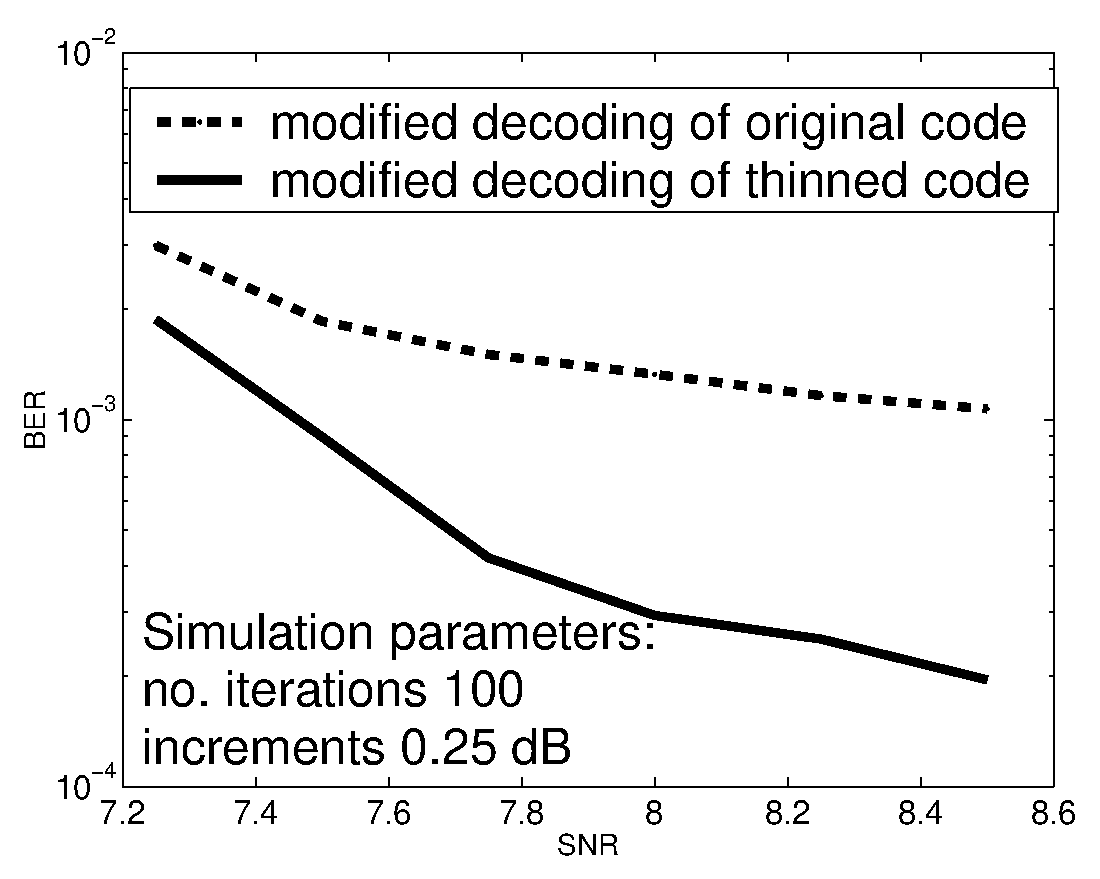
\includegraphics[width=2.5in,height=1.18in]{fig233b.eps}
\caption{Performance of LDPC (529,462) over AWGN with one
repetition} \vspace{-0.05in}
\end{figure}



\section{Concluding remarks}
We proposed a technique for modifying array-based LDPC codes when
varying sampling rate may cause repetition of symbols. Allowing a
small loss in rate, we systematically expurgate the code to get a
thinned code with significantly improved synchronization error
correction properties. We also gave a scheme for constructing
$t$-repetitions correcting families of sequences. Incorporating
multiple synchronization error correction capabilities in
array-based LDPC codes and other codes of interest is a topic for
future research.

% conference papers do not normally have an appendix

% use section* for acknowledgement
\vspace{-0.1in}
\section*{Acknowledgment}
% optional entry into table of contents (if used)
%\addcontentsline{toc}{section}{Acknowledgment}
The authors would like to thank Marvell Semiconductor Inc. and
U.C. MICRO program for supporting their research.



\begin{thebibliography}{17}

%\bibitem{Shannon1948}
%C. E. Shannon, ``A mathematical theory of communication,''
%\emph{Bell Syst.\ Tech.\ J.}, vol.\ 27, pt.~I, pp.~379--423, 1948;
%     pt.~II, pp.~623--656, 1948.
\bibitem{aji}
S. Aji and R. McEliece, ``The generalized distributive law",
\emph{IEEE Trans.  Inform. Theory} vol.\ 46(2), pp.~325--43, March
2000.
%\bibitem{tam}
%P. Bhagawat, M. Uppal and G. Choi, ``FPGA based implementation of
%decoder for array low-density parity check codes,''%In \emph{Proc. of
%\emph{ ICASSP}, 2005, pp.~29--32.%, Philadelphia, PA, USA.
%\bibitem{bours:94}
%P.A.H. Bours, ``Construction of fixed-length insertion/deletion
%correcting runlength-limited codes,'' \emph{IEEE Trans. Inf.
%Theory}, vol.\ 40(6), pp.~1841--1856, Nov. 1994.
\bibitem{cmnv:03}
G. Chen, M. Mitzenmacher, C. Ng and N. Varnica, ``Concatenated
codes for deletion channels,'' \emph{Int. Symp. Inform. Theory},
2003, p.~218.%, Yokohama, Japan.
\bibitem{dmackay:01}
M.C. Davey and D.J.C. MacKay, ``Reliable communication over
channels with insertions, deletions and substitutions,''
\emph{IEEE Trans. Inf. Theory}, vol.\ 47(2), pp.~687--98, Feb.
2001.
\bibitem{techArray:06} L. Dolecek and V. Anantharam, ``On array-based LDPC codes in channels
with varying sampling rate,'' available at
www.eecs.berkeley.edu/\~{}dolecek/papers
\bibitem{techRM:06} L. Dolecek and V. Anantharam, ``Using Reed-Muller codes in channels with synchronization and substitution errors,'' available at www.eecs.berkeley.edu/\~{}dolecek/papers
\bibitem{ibm:02} % linear time encoding    dsl app
E. Eleftheriou and S. \"{O}l\c{c}er, ``Low density parity check
codes for digital subscriber lines,'' \emph{Int. Conf. on Comm.},
2002, pp.~1752--57.
\bibitem{fan}
J. L. Fan, ``Array-codes as low-density parity-check codes,''
\emph{Second Int. Symp. on Turbo Codes and Related Topics}, 2000,
pp.~543--46.
%\bibitem{ferr:97}
%H.C. Ferreira, W.A. Clarke, A.S.J. Helberg, K.A.S. Abdel-Ghaffar and
%A.J. Han Vinck, ``Insertion/deletion correction with spectral
%nulls,'' \emph{IEEE Trans. Inf. Theory}, vol.\ 43(2), pp.~722--732,
%March 1997.
\bibitem{klove:95}
T. Kl{\o}ve, ``Codes correcting a single insertion/deletion of a
zero or a single peak-shift,'' \emph{IEEE Trans. Inf. Theory},
vol.\ 41(1), pp.~279--83, Jan. 1995.
\bibitem{kbek:04}
P. Kovintavewat, J. R. Barry, M. F. Erden and E. Kurtas,
``Per-survivor timing recovery for uncoded partial response
channels,''\emph{Int. Conf. on Comm.}, 2004, pp.~2715--19.%, Paris,
%France.
\bibitem{lev:66}
V. I. Levenshtein, ``Binary codes capable of correcting deletions,
insertions and reversals,'' \emph{Sov. Phys.-Dokl.}, vol.\ 10(8),
pp.~707--10, Feb. 1966.
\bibitem{liu:02}
J. Liu, H. Song and B.V.K.V. Kumar, ``Symbol timing recovery for
low-SNR partial response recording channels,'' \emph{Globecom}
2002, pp. 1129--36.%, San Francisco, CA, USA.
\bibitem{mittel:02}
T. Mittelholzer, ``Efficient encoding and minimum distance bounds
of Reed-Solomon-type array codes,'' \emph{Int. Symp. Inform.
Theory}, 2002, p. 282.%, Lausanne Switzerland.
\bibitem{mcla:02}
A. R. Nayak, J. Barry and S. W. McLaughlin, ``Joint timing
recovery and turbo equalization for coded partial response
channels,'' \emph{IEEE Trans. On Magnetics}, vol.\ 38(5),
pp.~2295--97, Sept. 2002.
\bibitem{sloane:00}
N.J.A. Sloane, ``On single deletion correcting codes,'' 2000.
Available at http://www.research.att.com/\~{ }njas/doc/dijen.pdf
\bibitem{kumar:04} %mr app
H. Song and B.V.K.V. Kumar, ``Low density parity check codes for
partial response channels,'' \emph{IEEE Signal Proc. Magazine},
vol.\ 21(1), pp.~56--66, Jan 2004.
\bibitem{vt:65}
R. R. Varshamov and G.M. Tenengolts, ``Codes which correct single
asymmetric errors,'' \emph{Avtomatika i Telemehkanika}, vol.\
26(2), pp.~288--92,1965.
\bibitem[17]{yanghell:03}
K. Yang and T. Helleseth, ``On the minimum distance of array codes
as LDPC codes," \emph{IEEE Trans. Inf. Theory}, vol.\ 49(12),
pp.~3268--71, Dec. 2003.
\end{thebibliography}
